%% TVCG submission — VerbalVis
%% Compile: pdflatex main && bibtex main && pdflatex main && pdflatex main
%% Template: IEEEtran (journal mode) — TVCG accepts IEEEtran or VGTC styles.

\documentclass[journal]{IEEEtran}

\usepackage{cite}
\usepackage{graphicx}
\graphicspath{{png/}}
\usepackage{capt-of}
\usepackage{amsmath,amssymb,amsfonts}
\usepackage{algorithmic}
\usepackage{booktabs}
\usepackage{array}
\usepackage{url}
\usepackage{xcolor}
\usepackage{hyperref}
\hypersetup{colorlinks=true,linkcolor=blue,citecolor=blue,urlcolor=blue}

\begin{document}

% =====================================================================
% Title
% =====================================================================
\title{VerbalVis: Full-Duplex Conversational Visual Analytics for Analytical Intent Revision}

\author{Anonymous Author(s)%
\thanks{Manuscript submitted to IEEE Transactions on Visualization and Computer Graphics. Source code, prompts, and study materials will be made available upon publication.}}


\IEEEaftertitletext{%
\begin{center}
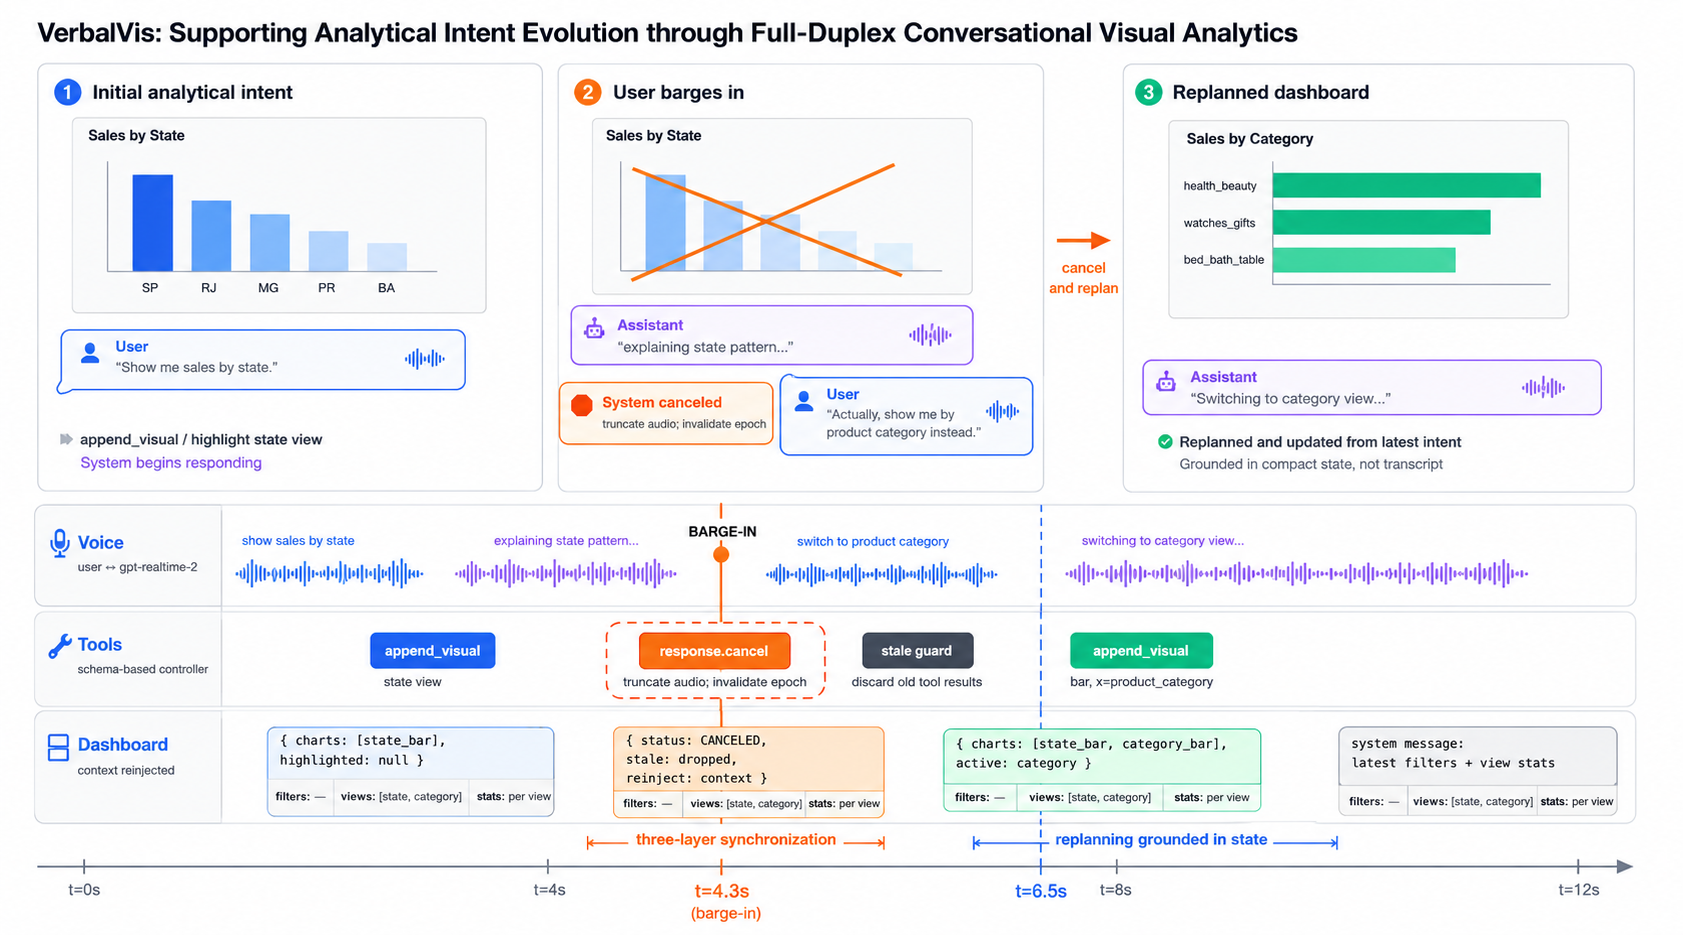
\includegraphics[width=\textwidth]{teaser-main.png}
\captionof{figure}{Overview of a barge-in episode in VerbalVis. While the assistant is explaining a visualization, the user interrupts to redirect the exploratory analysis from sales by state to sales by product category. VerbalVis immediately cancels obsolete speech, replans visualization actions through tool execution, reinjects the updated dashboard state as contextual grounding for the language model, and synchronously updates both the dashboard and spoken response. The aligned voice, tool, and dashboard timelines illustrate the coordinated full-duplex interaction that enables continuous analytical intent evolution without explicit turn switching.}
\label{fig:teaser}
\end{center}
}


\maketitle

% =====================================================================
% Abstract
% =====================================================================

\begin{abstract}
Exploratory data analysis is iterative: new observations may lead analysts to redirect questions, revise provisional explanations, or refine the data scope under investigation. Existing speech- and language-driven visual analytics systems generally support such changes only at discrete turn boundaries. Full-duplex interaction enables users to redirect an analysis while the assistant is still speaking, but stopping audio alone is insufficient when the superseded response may also have initiated actions that modify a persistent dashboard. We present \textbf{VerbalVis}, a full-duplex conversational visual analytics system that coordinates spoken output, schema-grounded tool execution, and dashboard state during mid-response redirection. Drawing on prior work in sensemaking and exploratory analysis, we use three non-exhaustive and potentially overlapping constructs---\emph{Analytical Goal Shift}, \emph{Working-Hypothesis Revision}, and \emph{Analytical Scope Refinement}---to characterize revision episodes. A lightweight formative study refined their operational boundaries and informed requirements for cancellation, state preservation, and visible feedback. VerbalVis truncates obsolete speech, invalidates superseded tool actions, discards stale results, and replans against the latest committed dashboard state. We evaluate it through an illustrative scenario and an exploratory within-subjects comparison of full-duplex and turn-based interaction.
\end{abstract}


\begin{IEEEkeywords}
Visual analytics, conversational interfaces, speech interaction, full-duplex dialogue, analytical intent, exploratory data analysis, large language models.
\end{IEEEkeywords}



\section{Introduction}
\label{sec:intro}

\IEEEPARstart{E}{xploratory} data analysis (EDA) is an iterative process in
which analysts move between observations, questions, provisional
explanations, and new analytical actions. Rather than executing a fully
specified plan, analysts often begin with incomplete information needs and
revise their direction as patterns, anomalies, and competing explanations
emerge~\cite{russell1993cost,pirolli2005sensemaking,
sacha2014knowledge,battle2019characterizing}. Such revisions may concern
different aspects of the investigation. An analyst may replace the primary
question being pursued, reconsider a working explanation, or restrict the
analysis to a more relevant population, period, region, or set of variables.
We use \emph{analytical intent revision} to refer to a local episode in which
the analyst supersedes, qualifies, or materially modifies an active analytical
commitment. Across an exploratory session, the accumulation of such episodes
constitutes the broader evolution of analytical intent.

Natural-language interfaces for visualization have made it increasingly
possible to express analytical operations through conversational commands.
Systems such as DataTone, Eviza, and NL4DV map language to data attributes,
filters, comparisons, aggregations, and visual specifications, while
multimodal systems combine language with pointing, touch, or direct
manipulation~\cite{gao2015datatone,setlur2016eviza,
narechania2021nl4dv,srinivasan2018orko,srinivasan2020inchorus}.
More recent LLM-powered visual analytics systems extend this interaction model
to data transformation, multistep planning, visualization generation, tool
execution, and conversational refinement
\cite{dibia2023lida,wang2024dataformulator2,zhao2024lightva,
weng2025insightlens}. These systems substantially increase the range of
analytical requests that can be expressed in language. However, interaction
generally remains organized around discrete handoff points: the user submits a
request, the system produces a response or completes a sequence of actions,
and the user subsequently provides a follow-up or correction.

This turn-based organization is particularly consequential for spoken
interaction because system output unfolds over time. While listening to an
assistant's explanation, an analyst may recognize that the system is pursuing
an irrelevant question, disagree with a tentative explanation, or identify a
more appropriate data subset. Requiring the analyst to wait until the current
response has finished separates the moment at which the analytical direction
changes from the moment at which the system can act on that change. Recent
full-duplex speech models provide a different interaction regime: the system
can continue listening while speaking, allowing the user to reclaim the floor
through barge-in. Yet barge-in alone does not solve the visual analytics
problem. Barge-in is a temporal event---the user begins speaking during system
output---whereas analytical revision is a semantic relation between the new
utterance and the currently active investigation. A user may interrupt only to
repair a recognition error, request clarification, or control the conversation;
conversely, a user may revise an analysis after waiting for the assistant to
finish.

More importantly, stopping audio does not necessarily stop the analytical
consequences of the superseded response. A conversational visual analytics
system may already have generated a tool call, initiated a database operation,
created a visualization specification, or scheduled a dashboard update. These
actions can complete after the user's latest utterance has redirected the
analysis. If their results are committed without checking whether the
originating response remains valid, the dashboard may continue to evolve
according to an obsolete intent even after the assistant has verbally
acknowledged the new request. Full-duplex conversational visual analytics
therefore introduces a state-consistency problem spanning three coupled
layers: spoken output, analytical tool execution, and persistent visualization
state. Supporting interruption at the audio layer is insufficient unless
response-dependent analytical work can also be invalidated and the revised
request can be interpreted against the latest valid dashboard state.

We present \textbf{VerbalVis}, a full-duplex conversational visual analytics
system designed to support analytical redirection while system speech and
analytical actions are still unfolding. VerbalVis integrates a real-time
speech model with schema-grounded visualization tools and a persistent
dashboard. When new user speech begins during an active response, the system
immediately stops local audio playback and requests cancellation of the
obsolete response. Each response and its associated tool actions are bound to
an execution epoch. A redirection advances the current epoch, causing tool
results associated with superseded responses to be rejected rather than
committed to the dashboard. After the redirecting utterance is interpreted,
VerbalVis replans from the latest committed dashboard state, including active
filters, highlights, and visualizations. A compact representation of this
state is reinjected as conversational context so that subsequent speech and
tool execution remain grounded in what the analyst currently sees.

VerbalVis does not introduce a new speech model or interruption detector.
Its contribution lies in the visual-analytics-specific orchestration required
to make full-duplex redirection coherent across speech, computation, and
visual state. In particular, the system treats the latest valid request as
potentially superseding an unfolding response and coordinates speech
truncation, response cancellation, stale-action invalidation, late-result
rejection, and dashboard-state-grounded replanning. This mechanism is agnostic
to the particular reason for the redirection: VerbalVis does not classify
revision types at runtime, and all superseded response work is governed by the
same response-lifecycle and state-validity safeguards.

To inform the design and analysis of this interaction, we draw on prior work
in sensemaking, scientific reasoning, information seeking, and exploratory
visual analysis. These traditions independently describe evolving analytical
goals, revisable hypotheses or explanatory frames, and progressive focusing
of broad information needs
\cite{pirolli2005sensemaking,klein2007dataframe,
klahr1988dual,bates1989berrypicking,vakkari2001changes,
battle2019characterizing}. We synthesize these traditions into three
theory-informed objects of analytical revision:
\emph{Analytical Goal Shift}, in which the primary analytical question or
desired knowledge outcome is materially reoriented;
\emph{Working-Hypothesis Revision}, in which a provisional explanation is
rejected, replaced, or qualified; and
\emph{Analytical Scope Refinement}, in which constraints over the relevant
population, time period, geography, variables, categories, granularity, or
data subset are changed while the broader objective is generally preserved.
These constructs are non-exhaustive and potentially overlapping. They provide
a vocabulary for formative inquiry, behavioral coding, and design discussion,
rather than a universal taxonomy of EDA behavior or a set of runtime intent
classes.

We conducted a lightweight formative design study with four participants
experienced in data analysis. The study did not attempt to derive or validate
a comprehensive taxonomy. Instead, it used the three constructs as
theory-informed sensitizing concepts to examine how analytical redirection is
expressed in speech, which aspects of prior context users expect to preserve,
which obsolete actions they expect the system to cancel, and which dashboard
operations are needed to enact a revised direction. The sessions also exposed
important boundary cases, including recognition repair, ordinary follow-up,
requests for additional evidence, and changes to analytical method or visual
representation. These observations refined the operational definitions used
in our analysis and informed requirements for semantic interpretation,
cross-layer cancellation, state-grounded replanning, visible execution state,
and recoverable dashboard manipulation.

We evaluate VerbalVis through an illustrative usage scenario and an exploratory
within-subjects mixed-methods study with eight participants. The study compares
a \emph{Full-Duplex} condition, in which users may speak while the assistant is
responding, with an otherwise matched \emph{Turn-Based} condition, in which
users must wait for the current response to finish. Both conditions use the
same model, voice, dashboard, analytical tools, tasks, and initial state. We
examine system responsiveness and state consistency, perceived control,
interaction flow, workload, exploratory behavior, analytical outcomes, and
the ways in which participants naturally revise an ongoing analysis. The
three analytical revision constructs are used to characterize observed
episodes, but the study is designed to evaluate the interaction and
orchestration mechanism rather than to validate the constructs as a universal
classification.

\textbf{Contributions.}
\begin{enumerate}
\setlength{\itemsep}{0pt}
\setlength{\parskip}{0pt}

\item A theory-informed characterization of analytical revision in
conversational visual analysis, distinguishing changes to the analytical
goal, working hypothesis, and analytical scope, together with formative
design evidence and requirements for supporting mid-response redirection.

\item VerbalVis, a full-duplex conversational visual analytics system that
coordinates speech truncation, response supersession, schema-grounded tool
execution, stale-result invalidation, and replanning against the latest
committed dashboard state.

\item An exploratory mixed-methods evaluation comparing full-duplex and
turn-based speech interaction in open-ended visual analysis, examining
interaction responsiveness, perceived control, workload, exploratory
behavior, and analytical outcomes.

\end{enumerate}





\section{Related Work}
\label{sec:related}

VerbalVis lies at the intersection of natural-language interaction for
visualization, LLM-powered visual analytics, full-duplex spoken dialogue, and
research on sensemaking and analytical revision. Prior work in these areas
provides important foundations for language grounding, multimodal interaction,
agent planning, interruption handling, and the representation of evolving
analysis. However, these capabilities have largely been studied separately.
VerbalVis focuses on their coordination when a spoken request semantically
supersedes an active response whose speech, analytical actions, and dashboard
updates may still be unfolding.

\subsection{Natural-Language Interaction for Visualization}
\label{sec:rw-nli}

Visualization-oriented natural-language interfaces (V-NLIs) seek to translate
user utterances into references to data attributes, values, analytical tasks,
and visual encodings. Early systems established that language could serve as
more than a textual shortcut to chart construction. DataTone, for example,
represents alternative interpretations through interactive ambiguity widgets,
allowing users to inspect and resolve underspecified mappings rather than
silently accepting a single parse~\cite{gao2015datatone}. Eviza grounds
utterances in both the underlying dataset and the active visualization,
supporting references to visible marks, filters, aggregations, and contextual
follow-up questions~\cite{setlur2016eviza}. NL4DV generalizes this translation
process into a reusable toolkit that extracts data attributes and analytical
tasks and produces candidate visualization specifications
\cite{narechania2021nl4dv}. Together, these systems establish language
grounding, ambiguity management, and contextual interpretation as central
requirements for conversational visual analysis.

Subsequent work expands language interaction through multimodal input and
richer conversational context. Orko combines speech and direct manipulation
for network exploration, enabling users to express analytical operations
through complementary modalities~\cite{srinivasan2018orko}. InChorus develops
a systematic vocabulary of operations, targets, parameters, and instruments
for interactions combining speech, pen, and touch across visualization types
\cite{srinivasan2020inchorus}. DataBreeze similarly interweaves spoken language
with direct manipulation over flexible unit visualizations, allowing users to
alternate between systematically encoded views and manually arranged visual
structures~\cite{srinivasan2021databreeze}. Snowy and conversational extensions
to NL4DV further investigate follow-up utterances, context-dependent
references, and the modification of existing views
\cite{srinivasan2021snowy,mitra2022conversational}. These systems demonstrate
that speech can complement visual interaction and that later utterances can be
interpreted relative to earlier dialogue and visualization state.

Other V-NLIs address increasingly complex analytical questions. FlowSense
integrates natural language into a dataflow environment, grounding requests in
the structure and state of an analytical workflow. Talk2Data decomposes complex
questions into simpler analytical requests and presents their answers through
multiple annotated visualizations~\cite{guo2021talk2data}. Such systems move
beyond one-shot chart generation toward contextual and multi-step analysis.
Nevertheless, conversational refinement is generally organized around
completed input and output units: an utterance is interpreted, a visualization
or response is produced, and the user subsequently refines the result.
Multimodal input may reduce the effort required to express an operation, but
speech is usually treated as an alternative or complementary command channel
rather than as a continuously available channel through which an unfolding
response can be superseded.

This distinction matters because modifying an analysis after a response has
completed is different from redirecting it while speech and computation are
still active. Existing V-NLIs provide important mechanisms for language
grounding, ambiguity resolution, follow-up interpretation, and multimodal
reference. They do not, however, generally specify how a new spoken request
should invalidate response-dependent actions that have already been generated
but have not yet been committed to a persistent dashboard. VerbalVis builds on
their contextual grounding and schema-based execution, but shifts attention
from turn-level refinement to the lifecycle of an active analytical response.

\subsection{LLM-Powered and Agentic Visual Analytics}
\label{sec:rw-agentic}

Large language models expand conversational data analysis from mapping
utterances to individual visual specifications toward data transformation,
code generation, multistep planning, tool execution, and insight
interpretation. LIDA decomposes visualization generation into stages for data
summarization, goal generation, visualization creation, and evaluation
\cite{dibia2023lida}. Data Formulator combines natural-language concepts with
directly specified visual encodings, allowing an LLM to synthesize the data
transformations required to instantiate a user-defined visualization
\cite{wang2024dataformulator}. Data Formulator~2 extends this approach to
iterative visualization authoring by supporting blended natural-language and
interface input, the reuse of prior designs, and navigation through a branching
history of data and chart variants~\cite{wang2024dataformulator2}. DynaVis
similarly augments generated visualizations with persistent editing controls,
supporting continued refinement beyond the initial prompt
\cite{vaithilingam2024dynavis}.

Agentic visual analytics systems further delegate analytical planning and
execution to LLM-based components. InsightPilot and related systems use
language models to recommend or conduct sequences of data-analysis operations
rather than generating only a single chart~\cite{ma2023insightpilot}. LightVA
organizes analysis through planner, executor, and controller components that
translate high-level analytical goals into lower-level tasks, visualizations,
and insights~\cite{zhao2024lightva}. Its task-flow representation also gives
users a means to inspect and manage the developing analytical plan.
ProactiveVA extends agent assistance from reactive question answering toward
context-sensitive intervention based on the user's ongoing interaction
history~\cite{zhao2025proactiveva}. These systems demonstrate how LLM agents
can participate in the planning and execution of visual analysis rather than
merely serving as language parsers.

A related line of work improves the inspectability and steerability of
LLM-mediated analysis. WaitGPT transforms generated analysis code into an
incrementally presented visual representation through which users can inspect,
verify, and modify individual operations while an analysis is being produced
\cite{xie2024waitgpt}. InsightLens records, organizes, and links insights,
visualizations, code, and conversational context to support navigation through
an extended LLM-assisted analysis~\cite{weng2025insightlens}. Sensecape and
other nonlinear conversational interfaces allow users to branch, spatially
organize, and revisit conversational material rather than preserving a single
linear transcript~\cite{suh2023sensecape}. These systems respond to limitations
of monolithic chat interfaces by externalizing intermediate reasoning,
analytical history, and alternative branches.

This work establishes several capabilities required by VerbalVis:
LLM-generated analytical plans, schema- or code-based execution, persistent
artifacts, history management, and user steering. However, steering is
typically expressed through text, graphical controls, or intervention at an
inspectable checkpoint. Even when intermediate operations are streamed, the
interaction model need not address concurrent spoken overlap or the
possibility that a late result from a superseded response will modify the
current dashboard. Branching histories preserve alternatives, while
provenance views make prior steps inspectable, but neither capability by itself
defines which in-flight actions remain authorized to commit after the user has
changed direction.

VerbalVis therefore addresses a complementary orchestration problem. It does
not seek to improve general-purpose LLM planning or autonomous visualization
generation. Instead, it binds generated analytical actions to the lifecycle of
the response that produced them. When that response is superseded, associated
actions become stale, and their results are prevented from modifying the
dashboard. This connects conversational steering to explicit state-validity
semantics across speech, tools, and visual output.

\subsection{Full-Duplex Conversational AI and Interruption}
\label{sec:rw-duplex}

Spoken interfaces vary in how they coordinate listening and speaking.
Push-to-talk and conventional turn-based systems separate user and system
audio into discrete turns. Streaming systems may incrementally recognize or
generate speech, but streaming alone does not imply that the system listens
and speaks concurrently. In a full-duplex system, user and assistant audio can
overlap: the system continues processing incoming speech while producing its
own output and must decide whether the input is background noise, a
backchannel, conversational overlap, or an attempt to take the floor
\cite{skantze2021turntaking}.

Barge-in has long been studied in spoken-dialogue systems as the ability to
detect user speech during system output and stop or modify the current
response~\cite{heins1997bargein}. Incremental dialogue research further shows
that partial recognition hypotheses and dialogue interpretations may be
revised as additional speech arrives~\cite{schlangen2011general}. More recent
full-duplex speech systems model concurrent input and output streams, natural
overlap, backchannels, echo cancellation, and context-sensitive interruption
\cite{lin2022duplex,wang2024fullduplex,veluri2024syncllm,
defossez2024moshi,yu2025salmonnomni}. These systems substantially improve the
temporal coordination of machine conversation by reducing dependence on rigid
end-of-turn detection.

HCI research also demonstrates that interruption policy shapes conversational
experience. Systems that ignore legitimate barge-in can make users feel
constrained by machine-controlled turns, whereas overly aggressive
interruption may terminate useful output in response to acknowledgements,
noise, or hesitation. Studies of turn-taking and interruption therefore
consider timing, floor management, responsiveness, and perceived control
\cite{cumbal2024finish,skantze2021turntaking}. Conversation analysis provides
an additional distinction between interruption and repair: repair practices
address trouble in speaking, hearing, or understanding, and do not necessarily
change the underlying task or informational goal
\cite{schegloff1977preference}.

These distinctions are essential for conversational visual analytics.
Barge-in is an observable timing event, while analytical revision concerns the
semantic relationship between a new utterance and the active investigation. A
user may barge in to acknowledge the assistant, correct a recognition error,
request repetition, or ask the assistant to stop speaking without changing the
analysis. Conversely, the user may wait until a response ends and then revise
the analytical goal, explanation, or scope. Interruption timing and analytical
revision should therefore be represented and evaluated separately.

Existing full-duplex research primarily addresses the speech layer: whether
the system continues listening, when it yields the floor, and how generated
audio is truncated or resumed. In visual analytics, however, a spoken response
may be coupled to database queries, visualization generation, filtering, or
other persistent state changes. Audio cancellation does not imply
computational cancellation, and computational cancellation does not guarantee
that a result already in transit will not be rendered. VerbalVis extends
full-duplex interaction from conversational floor management to analytical
state management. Speech onset can conservatively suspend obsolete output,
while response identifiers and execution epochs determine whether associated
tool results remain valid when they later reach the dashboard.

\subsection{Sensemaking and Analytical Revision}
\label{sec:rw-sensemaking}

Sensemaking and exploratory-analysis research provides the theoretical
foundation for treating analytical direction as revisable. Russell et al.
describe sensemaking as the construction and adaptation of representations
that support task-specific questions, emphasizing the costs of searching for,
instantiating, and shifting among representations
\cite{russell1993cost}. Pirolli and Card model intelligence analysis as
iterative movement between information foraging and sensemaking activities,
including the collection of evidence, construction of schemas, generation of
hypotheses, and development of a final representation
\cite{pirolli2005sensemaking}. In visual analytics, Sacha et al. similarly
describe knowledge generation through interacting exploration, verification,
and reasoning loops in which findings may generate new questions or support,
qualify, and falsify hypotheses~\cite{sacha2014knowledge}. These models do not
treat analysis as the execution of a fixed initial plan.

Prior work offers distinct foundations for changes to analytical goals,
working explanations, and scope. Empirical and theoretical accounts of
information seeking show that initial needs are often incomplete and evolve as
information is encountered. Bates' berrypicking model describes search as a
sequence of evolving queries rather than the execution of one stable
formulation~\cite{bates1989berrypicking}. Vakkari shows how broad information
needs become increasingly focused as a research problem develops
\cite{vakkari2001changes}. In exploratory visual analysis, Battle and Heer
synthesize evidence that analysts begin with goals of varying specificity,
refine them through interaction, and decompose open-ended analysis into more
focused subtasks~\cite{battle2019characterizing}. These accounts support the
possibility of an \emph{Analytical Goal Shift}, while also showing that a
complete replacement of the primary question must be distinguished from
incremental goal refinement or a change in strategy.

Hypothesis and frame revision provide a second foundation. Data--Frame Theory
describes sensemaking as a reciprocal process in which data are interpreted
through an explanatory frame and the frame is elaborated, questioned,
compared, or replaced as new evidence is encountered
\cite{klein2007dataframe}. Scientific-reasoning research distinguishes search
within a hypothesis space from search for experiments or evidence used to
evaluate those hypotheses~\cite{klahr1988dual}. This distinction separates a
change in explanation from a request for another visualization or test.
Research on anomalous evidence further shows that conflicting observations
can lead to theory revision, but may also be ignored, reinterpreted, or judged
insufficient~\cite{chinn1993anomalous}. We therefore use
\emph{Working-Hypothesis Revision}, rather than hypothesis correction, to
avoid implying that the newly proposed explanation is necessarily true.

A third foundation concerns progressive focusing and changes to the data
target. Information-foraging models describe the selection of increasingly
promising information patches, while search and visualization systems support
the progressive specification of facets, populations, variables, and
constraints~\cite{pirolli1999information,bates1989berrypicking,
vakkari2001changes}. Brehmer and Munzner's distinction among the analytical
\emph{why}, interaction \emph{how}, and data \emph{what} helps separate a
change in analytical purpose from a change in the data to which that purpose
applies~\cite{brehmer2013multi}. We use \emph{Analytical Scope Refinement} for
changes to population, time, geography, variables, categories, granularity, or
data subset that generally preserve the higher-level objective. Filtering is
one possible implementation of such a revision, but a filter operation is not
itself sufficient evidence that the analyst has semantically revised the
scope.

Analytical provenance and history systems capture how such reasoning unfolds.
Provenance frameworks distinguish histories of data, visualization state,
interaction, and reasoning and support review, communication, recovery, and
reproducibility~\cite{ragan2016characterizing}. SensePath combines interaction
logs with think-aloud data to reconstruct sensemaking processes
\cite{nguyen2016sensepath}, while graphical histories and branching systems
support revisiting prior states and pursuing alternatives
\cite{heer2008graphical,derthick2001branching}. This work is complementary to
VerbalVis: provenance records or reconstructs revisions that have occurred,
whereas VerbalVis must determine in real time whether an in-flight action still
belongs to the current analytical trajectory.

Taken together, these traditions establish that exploratory analysis can
involve evolving goals, revisable explanatory commitments, and progressively
refined data focus. They do not establish a universal three-part taxonomy.
VerbalVis synthesizes these literatures into three theory-informed,
non-exhaustive, and potentially overlapping objects of analytical revision:
\emph{Analytical Goal Shift}, \emph{Working-Hypothesis Revision}, and
\emph{Analytical Scope Refinement}. The constructs guide the formative study,
behavioral coding, and design discussion; they are not runtime classes used to
select separate system mechanisms. The unresolved systems question is how a
conversational VA environment should remain coherent when any such revision is
expressed while speech, analytical tools, and persistent visual state are
still active. VerbalVis addresses this gap through response supersession,
stale-action invalidation, and replanning from the latest committed dashboard
state.



\section{Formative Study and Design Requirements}
\label{sec:formative}

We conducted a lightweight formative design study to understand how analysts
express changes in analytical direction during spoken visual analysis and how
a conversational visual analytics system should respond when such changes
occur. The study was design-oriented rather than confirmatory. It did not aim
to discover an exhaustive taxonomy of exploratory behavior, validate a
cognitive model, or estimate the prevalence of different revision forms.
Instead, we used theory-informed concepts as starting points for examining
natural expressions of analytical revision, identifying compound and boundary
cases, and deriving requirements for coordinating speech, analytical actions,
and persistent dashboard state.

\subsection{Study Questions}
\label{sec:formative-questions}

The study addressed four formative questions:

\begin{description}
\item[\textbf{FQ1.}]
How do analysts express changes to their analytical goals, provisional
explanations, and data scope during spoken visual analysis?

```
\item[\textbf{FQ2.}]
When an active analytical response is redirected, what speech,
computational work, and dashboard state do users expect the system to
preserve, stop, invalidate, or update?

\item[\textbf{FQ3.}]
What boundary cases distinguish analytical revision from recognition
correction, conversational repair, ordinary follow-up, evidence seeking,
and changes to analytical method or visual representation?

\item[\textbf{FQ4.}]
Which dashboard operations are needed to enact revised analytical
directions through conversation?
```

\end{description}

We define an \emph{analytical revision episode} as a local interaction in
which an analyst supersedes, qualifies, or materially modifies an active
analytical commitment. The definition concerns the semantic relationship
between the latest utterance and the ongoing investigation; it does not require
the utterance to occur while the assistant is speaking.

\subsection{Theory-Informed Sensitizing Concepts}
\label{sec:formative-theory}

The formative inquiry was guided by three sensitizing concepts specified
before the sessions. They were synthesized from prior research on
sensemaking, exploratory visual analysis, scientific reasoning, information
seeking, and visualization tasks. The concepts were therefore not induced
solely from the four participants. We used the study to refine their
operational boundaries and design implications rather than to validate them
as a universal taxonomy.

\subsubsection{Analytical Goal Shift}

Sensemaking research characterizes analysis as an iterative process in which
people construct and adapt representations in response to task-specific
questions~\cite{russell1993cost}. Pirolli and Card similarly describe repeated
movement among information gathering, schema construction, hypothesis
generation, and the development of analytical products
\cite{pirolli2005sensemaking}. These general models establish that analytical
activity is not necessarily governed by one fixed plan, although they do not
themselves define a category called Goal Shift.

More direct support comes from research on evolving information needs and
exploratory goals. Bates' berrypicking model describes information seeking as
a sequence of evolving queries in which encountered information produces new
directions and reformulations~\cite{bates1989berrypicking}. Vakkari shows that
search behavior, relevance criteria, and the specificity of information needs
change as a research problem develops~\cite{vakkari2001changes}. In visual
analytics, Sacha et al.\ describe findings and insights as inputs to subsequent
exploration and verification loops~\cite{sacha2014knowledge}. Battle and Heer
further synthesize evidence that exploratory visual analysis may begin with
broad or underspecified goals that become refined, decomposed, or redirected
through interaction with data~\cite{battle2019characterizing}. Lam et al.
distinguish high-level analysis goals from the concrete tasks used to achieve
them~\cite{lam2018bridging}.

Building on these accounts, we use \emph{Analytical Goal Shift} for the
stronger case in which an analyst supersedes or materially reorients the
primary analytical question or desired knowledge outcome. For example,
``I care more about customer ratings than sales'' changes what the analyst
ultimately seeks to understand. In contrast, changing a chart type, sorting a
view, or selecting another analytical procedure does not by itself constitute
a goal shift because these changes may preserve the analytical purpose.

\subsubsection{Working-Hypothesis Revision}

The strongest and most direct theoretical foundation concerns the revision of
provisional explanations. Data--Frame Theory describes sensemaking as a
reciprocal relationship between observations and an explanatory frame. As new
evidence is encountered, a frame may be elaborated, questioned, compared with
alternatives, or replaced~\cite{klein2007dataframe}. Pontis and Blandford
provide empirical support for the development and modification of frames
during information-based sensemaking~\cite{pontis2016influence}.

Scientific-reasoning research makes an additional distinction between search
within a hypothesis space and search within an experiment or evidence space
\cite{klahr1988dual}. This distinction is important for our coding: changing
an explanation is not equivalent to requesting another visualization or test
of the same explanation. Research on anomalous evidence further shows that
conflicting observations can prompt theory revision, but may also be ignored,
reinterpreted, or judged insufficient~\cite{chinn1993anomalous}. Explanatory
coherence similarly concerns the evaluation of competing explanations rather
than the automatic identification of an objectively correct account
\cite{thagard1989explanatory}.

Visual-analytics research also treats hypothesis generation, verification,
and falsification as central components of knowledge generation
\cite{sacha2014knowledge}. Systems supporting analytical reasoning externalize
relationships among hypotheses, claims, and evidence
\cite{shrinivasan2008supporting}, while empirical work on hypothesis
formalization shows that conceptual hypotheses, variables, proxies, and
statistical implementations may be iteratively reconsidered
\cite{jun2022hypothesis}.

We therefore use \emph{Working-Hypothesis Revision}, rather than
\emph{Hypothesis Correction}, for an episode in which the analyst rejects,
replaces, qualifies, or materially alters a provisional explanation or causal
interpretation. The term \emph{working} emphasizes that the revised explanation
remains tentative. For example, `I think the low ratings are caused by
delivery delays rather than product quality'' revises the active explanation.
In contrast, `show me more evidence about delivery delays'' requests further
evaluation without necessarily changing the working hypothesis.

\subsubsection{Analytical Scope Refinement}

A third literature stream describes progressive focusing and the increasing
specification of initially broad information needs. Information Foraging
Theory explains how people allocate attention to promising information patches
and reduce the effective search space as information scent develops
\cite{pirolli1999information}. Bates and Vakkari describe the progressive
reformulation and specification of queries as users acquire a clearer
understanding of their problem
\cite{bates1989berrypicking,vakkari2001changes}. Battle and Heer similarly
describe exploratory visual analysis as moving between open-ended exploration
and more focused questions or subtasks
\cite{battle2019characterizing}.

Visualization task research provides a structural basis for distinguishing
scope from analytical purpose. Brehmer and Munzner separate the analytical
\emph{why}, the interaction \emph{how}, and the data \emph{what}
\cite{brehmer2013multilevel}. Lam et al.\ likewise distinguish broad analysis
goals from concrete tasks such as identifying a relevant population or
gathering particular evidence~\cite{lam2018bridging}. Voyager provides
design-oriented support for progressive focus through faceted browsing and
partial specification of data and visual properties
\cite{wongsuphasawat2016voyager}.

These works do not establish Analytical Scope Refinement as a named cognitive
category. Rather, they support the underlying phenomenon that analysts
progressively specify or alter the data target to which an analytical purpose
applies. We operationalize \emph{Analytical Scope Refinement} as a change in
constraints over the relevant population, time period, geographic region,
variables, categories, granularity, or data subset while the primary
analytical objective is generally preserved. Scope narrowing is one subtype;
scope broadening, substitution, and changes in granularity are also included.

For example, ``continue investigating low ratings, but only for S~ao Paulo''
preserves the higher-level question while changing its data target. A filter
operation is not automatically a scope revision: temporary filtering used to
inspect evidence may implement the current plan without changing the intended
scope of subsequent reasoning.

\begin{table*}[t]
\centering
\caption{Theoretical foundations of the sensitizing concepts used in the
formative study. Prior work supports the underlying objects of change, whereas
their organization as three constructs is our synthesis and operationalization
for conversational visual analytics rather than a previously established
taxonomy.}
\label{tab:revision-foundations}
\small
\begin{tabular}{
p{0.18\textwidth}
p{0.25\textwidth}
p{0.24\textwidth}
p{0.26\textwidth}}
\toprule
\textbf{Construct} &
\textbf{Literature foundation} &
\textbf{What prior work supports} &
\textbf{Operational boundary in this work} \
\midrule

\textbf{Analytical Goal Shift} &
Sensemaking, evolving queries, goal evolution, question formulation, and
goal--task decomposition
\cite{russell1993cost,pirolli2005sensemaking,
bates1989berrypicking,vakkari2001changes,
sacha2014knowledge,battle2019characterizing,
lam2018bridging} &
Questions and goals may evolve, become more specific, or open new lines of
inquiry as information is encountered. &
The primary question or desired knowledge outcome is superseded or materially
reoriented. Changes only to visualization, procedure, or interaction strategy
are excluded. \

\textbf{Working-Hypothesis Revision} &
Data--Frame Theory, scientific hypothesis search, anomalous evidence,
explanatory coherence, and hypothesis management
\cite{klein2007dataframe,pontis2016influence,
klahr1988dual,chinn1993anomalous,
thagard1989explanatory,sacha2014knowledge,
shrinivasan2008supporting,jun2022hypothesis} &
Provisional explanations can be generated, evaluated, qualified, compared,
rejected, and replaced. &
The explanatory proposition changes. Requests for more evidence that preserve
the active explanation are excluded. \

\textbf{Analytical Scope Refinement} &
Information foraging, progressive focusing, query refinement, data-target
specification, and faceted exploration
\cite{pirolli1999information,bates1989berrypicking,
vakkari2001changes,battle2019characterizing,
brehmer2013multilevel,lam2018bridging,
wongsuphasawat2016voyager} &
Broad information needs can become focused through the specification of
populations, facets, variables, constraints, and levels of detail. &
The data target or its constraints change while the higher-level objective is
generally preserved. Routine filtering is excluded unless it changes the
intended scope of subsequent reasoning. \
\bottomrule
\end{tabular}
\end{table*}

\subsubsection{Relationships and Boundaries}

The three constructs operate on related but distinguishable objects.
Analytical Goal Shift concerns the desired knowledge outcome;
Working-Hypothesis Revision concerns an epistemic or explanatory commitment;
and Analytical Scope Refinement concerns the data target and constraints. The
constructs are not assumed to be mutually exclusive. One utterance may alter
several objects simultaneously. For example:

\begin{quote}
``Forget sales; only examine low-rated orders in S~ao Paulo because delivery
may be the problem.''
\end{quote}

This utterance includes a shift from sales to low ratings, a refinement from
the full dataset to low-rated orders in S~ao Paulo, and a working hypothesis
concerning delivery. Such an episode may therefore receive one primary code
and multiple secondary codes.

The constructs are also non-exhaustive. Changes to aggregation, metric,
statistical model, visual encoding, chart type, or interaction strategy may
constitute a \emph{Method or Representation Change} without changing the
analytical goal, working hypothesis, or scope. These cases were retained as
residual codes rather than forced into one of the three constructs.

Finally, analytical revision is distinct from barge-in and conversational
repair. Barge-in describes when user speech begins relative to system output
\cite{skantze2021turntaking}; analytical revision describes how the semantic
content of the new utterance relates to the active investigation.
Conversational repair addresses trouble in speaking, hearing, or understanding
\cite{schegloff1977preference}. A user may therefore interrupt to correct a
misrecognized place name without revising the analysis, or may wait until the
assistant finishes before changing the analytical goal.

\subsection{Participants and Apparatus}
\label{sec:formative-participants}

We recruited four participants (P1--P4) from
\textcolor{red}{[RECRUITMENT SOURCE]}. All participants had prior experience
with data analysis or visualization. They reported
\textcolor{red}{[RANGE]} years of data-analysis experience and regularly used
tools including \textcolor{red}{[ACTUAL TOOLS]}.
\textcolor{red}{[NUMBER]} participants had previously used conversational AI
for data-related tasks, and \textcolor{red}{[NUMBER]} had experience with
speech-based assistants. None had previously used VerbalVis.
Participants' prior familiarity with the Olist dataset was
\textcolor{red}{[NONE/LOW/MIXED]}.

The study used an early prototype of VerbalVis connected to the Olist Brazilian
e-commerce dataset. The initial dashboard presented five coordinated views:
monthly order volume, category-level sales, state-level distribution,
review-score distribution, and delivery-time statistics. The prototype
supported spoken requests and a preliminary subset of schema-grounded
dashboard operations.

Each session lasted approximately
\textcolor{red}{[XX--XX]} minutes. Participants received
\textcolor{red}{[COMPENSATION]}. The study was approved by
\textcolor{red}{[ETHICS BODY OR APPROPRIATE ETHICS STATEMENT]}.

\subsection{Procedure}
\label{sec:formative-procedure}

Each session consisted of five stages.

\paragraph{Introduction and training.}

The researcher introduced the dataset, dashboard views, and speech interface.
Participants completed a short practice activity involving filtering,
highlighting, and requesting an additional visualization. They were informed
that they could redirect the system while it was speaking, but the three
sensitizing concepts were not introduced to avoid prompting participants to
produce particular revision forms.

\paragraph{Open-ended exploration.}

Participants were asked to investigate
\textcolor{red}{[ACTUAL FORMATIVE TASK]} and pursue any patterns, questions,
or explanations they considered relevant. They could change direction at any
time and were not required to interrupt the assistant or produce a prescribed
number of revisions. We did not require continuous think-aloud because
verbalizing concurrent reasoning could interfere with natural speech
interaction. At the end of the activity, participants briefly summarized
their findings and analytical path.

\paragraph{Critical-incident replay.}

The researcher replayed selected moments in which the participant redirected,
corrected, stopped, or followed up on the assistant. For each incident, the
participant was asked:

\begin{itemize}
\item what they intended to change;
\item which prior analytical state should remain valid;
\item whether ongoing speech or analytical work should stop;
\item whether already completed dashboard changes should be preserved;
\item and how they determined whether the system had followed the latest
request.
\end{itemize}

\paragraph{Response-lifecycle scenario walkthrough.}

Participants examined short scenarios in which user speech occurred at
different points in an analytical response: while the assistant was speaking,
after a tool call had been created, during tool execution, and immediately
before a dashboard update. Scenarios included analytical redirection,
recognition correction, clarification, acknowledgement, evidence seeking, and
representation changes. Participants described how they expected the system
to respond and which pending actions should remain authorized to modify the
dashboard.

\paragraph{Operation elicitation and interview.}

Participants described the dashboard operations they expected to perform
through speech and identified actions that would be difficult to express,
inspect, or reverse. The interview also covered preferred interruption
behavior, visibility of system state, recovery from unintended actions, and
the relative importance of immediate cancellation and preservation of
completed analytical work.

We recorded system audio, participant speech, transcripts, screen activity,
dashboard state, tool events, and researcher notes. For each critical incident,
we retained the preceding request, active assistant response, pending
analytical actions, participant utterance, and resulting dashboard state.

\subsection{Data Analysis}
\label{sec:formative-analysis}

The analysis followed a hybrid deductive--inductive strategy. Analytical Goal
Shift, Working-Hypothesis Revision, and Analytical Scope Refinement were
specified before coding as theory-informed sensitizing concepts. We did not
assume that all observed behavior would fit these constructs. Open coding was
used to identify residual and boundary cases.

We segmented the recordings into candidate episodes whenever a participant
spoke in relation to an active analytical request, assistant explanation, or
dashboard operation. Each episode included sufficient context to interpret the
new utterance: the preceding user request, active assistant response, visible
dashboard state, pending tool actions, and resulting system behavior.
Conversation unrelated to the analytical activity was excluded.

The coding scheme included:

\begin{itemize}
\item \textbf{Analytical Goal Shift};
\item \textbf{Working-Hypothesis Revision};
\item \textbf{Analytical Scope Refinement};
\item \textbf{Method or Representation Change};
\item \textbf{Request for Additional Evidence};
\item \textbf{Automatic-Speech-Recognition Correction};
\item \textbf{Conversational Repair or Clarification};
\item \textbf{Ordinary Follow-Up};
\item \textbf{Non-Analytical Barge-In}; and
\item \textbf{Ambiguous or Unclassified}.
\end{itemize}

An episode could receive one primary code and zero or more secondary codes.
The primary code captured the change most necessary to interpret the latest
request. Secondary codes captured compound episodes involving multiple objects
of change. Interaction timing was coded independently as:

\begin{itemize}
\item during assistant speech;
\item after speech but before tool completion;
\item during tool execution;
\item after dashboard commitment; or
\item at an ordinary turn boundary.
\end{itemize}

Two researchers independently coded
\textcolor{red}{[ALL EPISODES OR THE ACTUAL PROPORTION]}. They first discussed
\textcolor{red}{[NUMBER]} training episodes to refine the codebook and then
coded the remaining material independently. Disagreements were resolved
through discussion with reference to the complete interaction context and
participants' replay explanations. Report
\textcolor{red}{[THE ACTUAL AGREEMENT PROCEDURE OR RELIABILITY STATISTIC ONLY
IF CALCULATED]}.

Given the formative purpose and small sample, analysis emphasized expressions,
boundary cases, user expectations, and design implications rather than
frequency comparisons or claims of theoretical saturation.

\subsection{Formative Findings}
\label{sec:formative-findings}

The analysis yielded \textcolor{red}{[NUMBER]} candidate episodes, including
\textcolor{red}{[NUMBER]} analytical revisions,
\textcolor{red}{[NUMBER]} repair or clarification episodes, and
\textcolor{red}{[NUMBER]} other follow-ups or control actions. We report the
results as design-oriented themes rather than estimates of the prevalence of
revision forms.

\subsubsection{Revisions superseded active analytical commitments}

Participants expressed redirection through language such as
\textcolor{red}{[INSERT ACTUAL EXPRESSIONS, E.G., `ACTUALLY,'' `NO,
INSTEAD,'' `I CARE MORE ABOUT,'' OR `ONLY LOOK AT'']}. Such utterances did
not merely add another operation; they indicated that some aspect of the
active analytical response should no longer guide subsequent speech or
dashboard updates.

For example, \textcolor{red}{[PARTICIPANT]} redirected the analysis from
\textcolor{red}{[OLD GOAL]} to \textcolor{red}{[NEW GOAL]}, stating,
``\textcolor{red}{[VERBATIM QUOTE]}.'' Another participant retained the
question concerning \textcolor{red}{[QUESTION]} but revised the explanation
from \textcolor{red}{[OLD HYPOTHESIS]} to
\textcolor{red}{[NEW HYPOTHESIS]}. Scope refinements changed
\textcolor{red}{[ACTUAL POPULATION/TIME/REGION/VARIABLE]} while preserving the
broader objective.

These incidents demonstrated the descriptive usefulness of distinguishing
the object of change, but they did not establish three exhaustive or mutually
exclusive revision types.

\subsubsection{Some revision episodes changed multiple objects}

Several utterances combined changes to analytical purpose, explanation, and
scope. For instance, \textcolor{red}{[PARTICIPANT]} stated,
``\textcolor{red}{[ACTUAL COMPOUND QUOTE]},'' which changed
\textcolor{red}{[GOAL]}, introduced \textcolor{red}{[SCOPE]}, and proposed
\textcolor{red}{[HYPOTHESIS]}.

These episodes motivated primary and secondary coding rather than
forced-choice classification. They also indicated that runtime classification
into three types was unnecessary: the system instead needed to identify the
latest valid request and prevent response-dependent obsolete work from
altering the dashboard.

\subsubsection{Stopping speech did not necessarily cancel analytical consequences}

When speech stopped but an earlier operation subsequently modified the
dashboard, participants described the behavior as
\textcolor{red}{[ACTUAL WORDING]}. They expected pending actions associated
with the superseded response either to be cancelled or prevented from
committing their results.

Participants distinguished pending work from dashboard changes that had
already been visibly committed. Completed and still-useful state could remain
available, whereas uncommitted results from a superseded response should not
appear after redirection. This distinction motivated an explicit separation
between the latest committed dashboard state and speculative in-flight work.

\subsubsection{Visible dashboard state determined whether the revision appeared successful}

Participants evaluated system understanding through visible filters,
highlights, view titles, and created or removed visualizations. A verbal
acknowledgement was insufficient when the dashboard continued to reflect the
previous request.

Participants requested clearer indications of
\textcolor{red}{[ACTUAL REQUESTED STATES, SUCH AS LISTENING, SPEAKING,
EXECUTING, OR CANCELLED]}. They also emphasized recoverability when a spoken
request produced an unintended state change.

\subsubsection{Barge-in did not necessarily indicate analytical revision}

The sessions contained interruptions that did not change the analytical goal,
working hypothesis, or scope. These included recognition correction,
clarification, acknowledgement, requests for additional evidence, and changes
to chart type or aggregation.

For example, `\textcolor{red}{[ACTUAL ASR-REPAIR QUOTE]}'' corrected the
system's recognition, while `\textcolor{red}{[ACTUAL EVIDENCE-REQUEST
QUOTE]}'' requested another test without modifying the active explanation.
These cases reinforced the need to separate speech timing from analytical
semantics.

\subsubsection{Participants requested operations over multiple dashboard targets}

Participant-elicited operations concerned four broad targets:

\begin{itemize}
\item \textbf{data scope}, including filters, aggregation, and comparison;
\item \textbf{view specification}, including chart type, encoding, sorting,
highlighting, and focus;
\item \textbf{dashboard organization}, including adding, moving,
replacing, and removing views; and
\item \textbf{analytical assistance}, including explaining a visualization
and summarizing the dashboard.
\end{itemize}

We consolidated these elicited needs with operations identified in established
visualization task and interaction frameworks
\cite{brehmer2013multilevel,yi2007toward} into the conversational dashboard
operation inventory in Table~\ref{tab:operation-inventory}. The inventory
documents a broader design space rather than an exhaustive taxonomy or a list
of capabilities fully implemented in VerbalVis. The current prototype
implements only the schema-grounded subset used in the subsequent evaluation.

\subsection{Design Requirements}
\label{sec:design-requirements}

The theoretical framing and formative findings informed five design
requirements.

\paragraph{DR1: Separate speech timing from analytical interpretation.}

The system should react promptly when user speech begins but should not assume
that every barge-in changes analytical intent. Speech onset may conservatively
suspend audio output, while the completed utterance is subsequently
interpreted as analytical revision, repair, clarification, evidence seeking,
representation change, or ordinary follow-up.

\paragraph{DR2: Coordinate cancellation across speech and analytical execution.}

When a new request supersedes an active response, cancellation should extend
beyond audio playback. Response-dependent tool calls, database operations,
visualization specifications, and pending dashboard updates must be cancelled
or marked stale so that they cannot later modify the visible state.

\paragraph{DR3: Replan from the latest committed dashboard state.}

The revised response should be grounded in the most recent valid filters,
highlights, views, and data scope. Speculative changes associated with a
superseded response should not become context for the new plan. The system
therefore requires an explicit distinction between committed dashboard state
and in-flight analytical work.

\paragraph{DR4: Make listening, execution, cancellation, and commitment visible.}

Users should be able to determine whether the system is listening, speaking,
executing an analytical action, cancelling obsolete work, or waiting for
input. The interface should expose the state that grounds subsequent
conversation and support recovery when an unexpected operation is committed.

\paragraph{DR5: Provide bounded, schema-grounded, and recoverable dashboard operations.}

Conversational interaction should expose a coherent set of operations over
data scope, visual specifications, dashboard organization, and analytical
assistance. Operations that modify persistent state should use explicit
schemas and support removal, replacement, or undo. The broader operation
inventory guides future extension, while the present prototype implements the
subset required to study full-duplex analytical redirection.

These requirements directly informed the architecture of VerbalVis. DR1
motivated the separation of speech-onset handling from semantic
interpretation. DR2 motivated response-bound execution epochs and stale-result
rejection. DR3 motivated dashboard versioning and compact state reinjection.
DR4 motivated visible listening and execution feedback. DR5 motivated the
schema-grounded tool layer described in Section~\ref{sec:system}.

\subsection{Scope of the Formative Evidence}
\label{sec:formative-limitations}

The formative study provides design-oriented evidence rather than validation
of a general theory of analytical intent. Four participants cannot establish
theoretical saturation, estimate population-level frequencies, or demonstrate
that the three sensitizing concepts cover all exploratory behavior. The
constructs may overlap, and revisions to method, metric, operationalization,
or visual representation may constitute additional objects of change.

Accordingly, we use the formative study to refine inclusion and exclusion
criteria, identify compound and residual cases, and derive requirements for
full-duplex conversational visual analytics. The subsequent user study
evaluates the interaction and orchestration mechanisms of VerbalVis; it does
not test the three constructs as a universal taxonomy.

% =====================================================================
\section{System Design and Implementation}
\label{sec:system}

\subsection{Design Goals}
The framework yields three design goals:
\begin{itemize}
\item \textbf{DG1: Continuous intent revision.} Support revision at any moment, not only at turn boundaries.
\item \textbf{DG2: Rapid replanning after supersession.} Once an interruption is detected during assistant output, the system must prevent stale response work from committing, interpret the redirecting utterance, and re-plan against current dashboard state with minimal added latency.
\item \textbf{DG3: Dashboard--intent synchrony.} The shared dashboard must always reflect the latest applied operations and must serve as the canonical source of truth for the LLM, so that explanations are grounded in what the user sees rather than in the model's prior outputs.
\end{itemize}

\subsection{Architecture Overview}
VerbalVis comprises a Vue~3 + Vega-Lite frontend, a FastAPI backend with an in-memory DuckDB analytics layer, and a relay that bridges a browser WebSocket to the OpenAI Realtime WebSocket (Fig.~\ref{fig:arch}). The backend exposes a single \texttt{/ws} endpoint; on connection, it constructs a \texttt{RealtimeSession} that runs two concurrent async loops --- one forwarding client audio frames to OpenAI, one demultiplexing OpenAI events to the client and dispatching tool calls.

\begin{figure}[t]
\centering
\fbox{\parbox{0.92\linewidth}{\centering\small
\textbf{[Figure placeholder]} System architecture: Frontend (Vue/Vega-Lite) $\leftrightarrow$ Backend (FastAPI relay + DuckDB) $\leftrightarrow$ OpenAI Realtime (\texttt{gpt-realtime-2}). Realtime Layer (audio streaming, VAD, barge-in, response cancel) on the left; Analytics Layer (tool calls, DuckDB, dashboard update) on the right; shared dashboard state in the middle.}}
\caption{VerbalVis architecture. The Realtime Layer handles conversational coordination; the Analytics Layer executes tool calls asynchronously and updates the dashboard state, which is reinjected as system context after every tool call.}
\label{fig:arch}
\end{figure}

\noindent\emph{Realtime layer.} \texttt{gpt-realtime-2} streams 24\,kHz PCM audio in both directions. Depending on the experimental condition, the frontend uses local voice gating or push-to-talk, while the Realtime session may also expose server-side speech events such as \texttt{input\_audio\_buffer.speech\_started} and \texttt{\dots speech\_stopped}. On interruption-relevant events, the backend increments a \emph{turn epoch}, records the in-flight \texttt{response\_id} as invalidated, and marks tool tasks from the cancelled response as stale. In push-to-talk mode the backend additionally sends \texttt{response.cancel}; in server-interruption mode, it relies on the Realtime session's native interruption behavior and applies the same stale-result discipline locally.

\noindent\emph{Analytics layer.} Tool calls (\texttt{response.function\_call\_arguments.done}) are dispatched to handlers backed by DuckDB queries. DuckDB holds two derived fact tables built from seven Olist CSVs at startup: \texttt{fact\_order} (one row per delivered order, carrying order-grain attributes including \texttt{order\_month}, \texttt{review\_score}, \texttt{customer\_state}, \texttt{delivery\_days}, and per-order payment) and \texttt{fact\_item} (one row per order item, additionally carrying \texttt{product\_category} and per-item revenue $\textrm{price} + \textrm{freight}$). The two-table design lets revenue retain the correct semantics under both order-grain and item-grain aggregations; cross-grain filters on \texttt{product\_category} from the order table are rewritten as \texttt{order\_id IN (SELECT \dots FROM fact\_item WHERE \dots)} subqueries by a shared \texttt{build\_where} helper.

VerbalVis employs real-time full-duplex audio interaction for conversational coordination, while analytical operations are executed asynchronously through tool calls that update the dashboard state.

\subsection{Tool Taxonomy}
Following the Brehmer--Munzner multi-level typology~\cite{brehmer2013multi} and Yi et al.'s how-axis~\cite{yi2007toward}, we organize VerbalVis operations along three dimensions: \emph{why} (analytical goal), \emph{how} (interaction primitive), and \emph{what} (target of the operation: data, view, layout, insight). Table~\ref{tab:tools} lists a 15-operation taxonomy for the design space. The current prototype realizes five dashboard operations end-to-end as schema-based tools: \texttt{filter\_data}, \texttt{remove\_filter}, \texttt{highlight\_visual}, \texttt{append\_visual}, and \texttt{delete\_visual}. This subset is deliberately narrow: it covers the operations needed for the running example and user-study tasks while keeping tool selection predictable under realtime interruption.

\begin{table*}[t]
\centering
\caption{VerbalVis Tool Taxonomy. Five operations are implemented end-to-end as schema-based tools (marked $\checkmark$); the remainder define the broader design space. \emph{Why} follows Brehmer--Munzner; \emph{How} follows Yi et al.; \emph{What} identifies the operation target.}
\label{tab:tools}
\small
\begin{tabular}{lllllc}
\toprule
\textbf{Tool} & \textbf{Why} & \textbf{Why-Detail} & \textbf{How} & \textbf{What} & \textbf{Impl.} \\
\midrule
\texttt{filter\_data}          & Discover & Locate     & Filter                 & Data    & $\checkmark$ \\
\texttt{remove\_filter}        & Discover & Locate     & Filter                 & Data    & $\checkmark$ \\
\texttt{aggregate\_data}       & Discover & Summarize  & Abstract/Elaborate     & Data    &              \\
\texttt{compare\_data}         & Discover & Compare    & Connect                & Data    &              \\
\texttt{change\_chart\_type}   & Discover & Explore    & Encode                 & View    &              \\
\texttt{change\_encoding}      & Present  & ---        & Encode                 & View    &              \\
\texttt{change\_sort}          & Discover & Compare    & Reconfigure            & View    &              \\
\texttt{highlight\_visual}     & Discover & Locate     & Select                 & View    & $\checkmark$ \\
\texttt{focus\_visual}         & Discover & Explore    & Select+Reconfigure     & View    &              \\
\texttt{append\_visual}        & Discover & Explore    & Encode                 & View    & $\checkmark$ \\
\texttt{move\_visual}          & Present  & ---        & Reconfigure            & Layout  &              \\
\texttt{delete\_visual}        & Discover & Identify   & Reconfigure            & Layout  & $\checkmark$ \\
\texttt{replace\_visual}       & Discover & Explore    & Reconfigure            & Layout  &              \\
\texttt{explain\_visual}       & Discover & Identify   & Connect                & Insight &              \\
\texttt{summarize\_dashboard}  & Discover & Summarize  & Abstract/Elaborate     & Insight &              \\
\bottomrule
\end{tabular}
\end{table*}

\noindent The implemented tools are deliberately minimal. \texttt{filter\_data} centralizes global dataset narrowing (with a \texttt{field=null} convention for clearing, an \texttt{append} flag for AND-accumulation, and operator support for \texttt{eq, neq, in, gte, lte, between}); \texttt{remove\_filter} removes one field constraint without disturbing the rest; \texttt{highlight\_visual} redirects attention without changing data; \texttt{append\_visual} creates a new chart at item or order grain based on whether \texttt{product\_category} appears in the encoding; and \texttt{delete\_visual} removes views from the shared workspace. This minimality is intentional: most analytical state changes in our scenarios can be expressed by composing these operations, which keeps the model's tool-selection decision tree shallow and reduces the surface area on which the LLM can hallucinate.

\subsection{Layered Prompt Design}
The system prompt is constructed in four labeled sections, in line with the prompt-structure recommendations of the GPT-realtime-2 prompting guide~\cite{openai_realtime_prompt}. \emph{Identity} fixes the assistant as a collaborative data analyst, instructs language mirroring, and prescribes the opening behavior (greet, introduce the Olist dataset, walk through the four base views, then invite the user to choose a direction --- explicitly without preemptively highlighting any view). \emph{Dashboard Knowledge} provides a bidirectional view-id $\leftrightarrow$ Chinese-and-English-label dictionary, the exhaustive field list (forbidding fabricated fields such as ``return\_rate'' or ``profit''), and value semantics (e.g., \texttt{review\_score} 1--2 negative; \texttt{customer\_state} two-letter codes; revenue in BRL pronounced ``reais''). \emph{Tool Usage Rules} specify operator semantics, the cross-grain filter convention, and tool-selection guidelines that explicitly forbid defaulting to the review view for generic prompts such as ``what is interesting in the data.'' \emph{Realtime Rules} legitimize interruption as a high-priority signal and instruct the model to abandon prior explanations and re-evaluate against the latest user utterance.

\subsection{Dashboard State and Context Reinjection}
The four base views (\texttt{view-trend}, \texttt{view-review}, \texttt{view-map}, \texttt{view-category}) and any user-added \texttt{workspace-N} charts are maintained as a single backend list. After every tool call, the backend (i) re-queries all views against the current filter set, (ii) recomputes per-view summary statistics (e.g., peak month, low-score ratio, top state, top category), (iii) pushes a \texttt{views\_update} event to the frontend for re-render, and (iv) injects a compact textual snapshot of the dashboard --- highlighted view, active filters, total filtered row count, and per-view summary --- back into the LLM as a \texttt{system} message. This \emph{context reinjection} pattern follows the guidance in the GPT-realtime-2 long-context section~\cite{openai_realtime_prompt}: the model is never asked to reconstruct dashboard state from prior turns, only to act on what it is given.

\subsection{Supersession Control Protocol}
VerbalVis treats barge-in as a control event, not as a semantic classifier. The reusable protocol has five stages. First, the runtime detects possible supersession through either a server speech-start event or a client push-to-talk start during assistant output. Second, the backend increments \texttt{turn\_epoch}, so newly arriving user input and later tool calls belong to a new response epoch. Third, the system attempts to stop obsolete output through \texttt{response.cancel} or \texttt{conversation.item.truncate}, depending on the input mode and Realtime event sequence. Fourth, tool calls associated with the superseded response are cancelled when possible and otherwise checked with \texttt{is\_stale\_tool\_call} before any result is returned to the model or applied to the dashboard. Fifth, VerbalVis reinjects a compact dashboard snapshot before the next \texttt{response.create}, so the revised plan is grounded in the latest valid visual state.

When barge-in is enabled, an interruption is represented by either a server speech-start event or a client push-to-talk start during assistant output. The backend then:
\begin{enumerate}
\item Increment the per-session \texttt{turn\_epoch}; record the in-flight \texttt{response\_id} as invalidated.
\item Cancel all in-flight tool tasks bound to the cancelled response.
\item Send \texttt{response.cancel} or \texttt{conversation.item.truncate} when the local input mode requires explicit cancellation or audio truncation.
\item Forward \texttt{speech\_started} to the frontend so the UI can stop playback immediately.
\end{enumerate}
A double-lock discipline (\texttt{openai\_send\_lock} for outbound messages, \texttt{tool\_state\_lock} for state mutation) and a per-response pending-tool counter ensure that (i) tool results from cancelled responses are discarded by an \texttt{is\_stale\_tool\_call} check before being forwarded to the model, and (ii) when a single model turn issues multiple tool calls, only the final completing call triggers a fresh \texttt{response.create}, preventing duplicate or racing responses.

\noindent\textbf{No-barge ablation.}
We define \textbf{VerbalVis-NoBarge} as the controlled ablation of the protocol. It uses the same \texttt{gpt-realtime-2} model, voice, prompt, tool schema, dashboard, backend, VAD settings, and context-reinjection logic as VerbalVis-FullDuplex. The only intended difference is policy: user speech during assistant output is recorded or queued, but it does not trigger \texttt{response.cancel}, \texttt{conversation.item.truncate}, epoch invalidation, or stale-tool discard until the current response completes. This condition separates the effect of the realtime model family from the specific effect of the supersession path.

% =====================================================================
\section{Case Study: Three Forms of Analytical Intent Revision}
\label{sec:case}

We illustrate the framework with a single session on the Olist Brazilian e-commerce dataset (96{,}478 delivered orders; 110{,}196 order items spanning 73 product categories and 27 states; September 2016 -- August 2018). The analyst, a domain non-expert, was asked to explore customer satisfaction with no predetermined goal.

\subsection{Initial State} The system greets the user, names the dataset, and walks through the four base views: monthly order trend, review-score distribution, orders by state, top-15 categories by revenue. The system then asks the analyst what they would like to explore. The analyst responds, ``Let's look at the trend.''

\subsection{Type 1 --- Goal Shift}
\emph{System (mid-utterance):} ``Order volume peaks in November 2017, roughly 4$\times$ the average month. Let me decompose that by product category to see whether it's a Black Friday effect across categories or concentrated in --- ''
\emph{Analyst (barge-in):} ``I care more about ratings, not sales.''

The barge-in fires \texttt{response.cancel}; the redirecting utterance is interpreted; the controller emits \texttt{highlight\_visual(view-review)} and the assistant continues: ``The review distribution is heavily concentrated at 5 stars but with a non-trivial 1- and 2-star tail. Want me to filter to low-rated orders and see what they share?'' The intent has shifted from a sales decomposition to a satisfaction investigation; the analyst was spared the remainder of the category breakdown.

\subsection{Type 2 --- Hypothesis Correction}
\emph{System (mid-utterance):} ``Electronics-adjacent categories such as \texttt{computers\_accessories} and \texttt{electronics} show below-average ratings. This is often attributable to product quality issues with --- ''
\emph{Analyst (barge-in):} ``It's logistics, not the products.''

The system invokes \texttt{append\_visual(scatter, delivery\_days, review\_score)} followed by \texttt{filter\_data(review\_score, lte, 2)}; the resulting scatter shows the low-rated tail clustering at high delivery days. The assistant continues: ``You're right --- low-rated orders disproportionately have delivery times above 20 days; the product-quality story doesn't hold up.'' The intent revision substituted a delivery hypothesis for a product-quality hypothesis, and the assistant aborted its prior explanation rather than completing it.

\subsection{Type 3 --- Scope Narrowing}
\emph{System (mid-utterance):} ``Among states with the worst delivery times, the northeast --- Bahia and Cear\'a --- have averages above 25 days, while --- ''
\emph{Analyst (barge-in):} ``Just S\~ao Paulo.''

\texttt{filter\_data(customer\_state, eq, "SP")} is issued; all four base views recompute against the SP-only subset; the assistant pivots to ``Within SP, average delivery is 8.4 days; the low-rated tail is much smaller than the national figure.'' Scope contracted from a national survey to a state-level focus, exploiting the analyst's prior interest in SP without the analyst having had to articulate that interest at the start of the session.

\subsection{Summary}
Each revision corresponds to one of the three framework types; the dashboard, the system narration, and the model's working hypothesis remained synchronized throughout because every superseded response was followed by a fresh \texttt{conversation.item.create} of dashboard context before the next \texttt{response.create}. We argue this synchrony is the practical value of treating barge-in as a structural supersession signal rather than merely as audio cancellation.

% =====================================================================
\section{User Study and Technical Benchmark}
\label{sec:study}

\subsection{Design}
The study is designed to test the paper's central claim rather than general usability: whether a full-duplex supersession pathway makes analytical intent revision in EDA faster, more natural, and more controllable. The primary causal comparison is \textbf{not} between a realtime speech model and a cascaded speech pipeline. Instead, we compare two conditions that share the same model, voice, prompt, tool schema, dashboard, backend, VAD configuration, and context-reinjection logic. The only intended difference is whether user speech during assistant output triggers immediate response cancellation, epoch invalidation, and stale-action discard.

We plan a within-subjects, counterbalanced study with $N{=}12$--$16$ participants. Participants must have basic data-analysis experience, but need not know the Olist domain in advance. Each participant completes two open-ended exploration tasks on the Olist dataset, one per primary condition; task--condition assignment and condition order are counterbalanced. Each task lasts 12--15 minutes after a short tutorial.

\begin{itemize}
\item \textbf{Condition A (VerbalVis-FullDuplex):} audio is handled by the \texttt{gpt-realtime-2} session; the user can speak during assistant output; barge-in cancels or truncates the current response, increments \texttt{turn\_epoch}, invalidates stale tool work, and triggers replanning against reinjected dashboard context.
\item \textbf{Condition B (VerbalVis-NoBarge):} the system uses the same \texttt{gpt-realtime-2} session, voice, prompt, VAD settings, dashboard, backend, tool schema, and context-injection logic. However, user speech during assistant output is queued until the current response completes; it does not trigger \texttt{response.cancel}, \texttt{conversation.item.truncate}, immediate epoch invalidation, or stale-tool discard. This preserves the realtime model family while removing the supersession policy.
\end{itemize}

\noindent\textbf{Supplementary ecological baseline.}
We additionally define \textbf{VerbalVis-Cascade} as an ecological baseline rather than the main causal comparison. In this condition, user speech is transcribed by ASR, passed to a text LLM using the same dashboard tool schema and Olist backend, and synthesized back to speech with TTS. The user must wait for the system to finish before the next request is processed. This baseline represents the speech-wrapped, turn-based text-LLM VA regime implicit in systems such as LightVA and DashChat, but it necessarily changes model type, speech pipeline, ASR/TTS latency, audio quality, turn-taking policy, and response timing. We therefore report Cascade results as supplementary context, not as evidence that the barge-in mechanism alone caused any observed advantage.

\subsection{Tasks}
Tasks are written to invite open-ended EDA while naturally eliciting the three revision types in our framework. Participants are not instructed to interrupt. The tutorial only explains the interaction regime of each condition: in FullDuplex they may speak whenever they want to redirect the analysis; in NoBarge their speech during assistant output is accepted but processed after the current response finishes. If Cascade is run, participants are told that it is a turn-based speech interface whose next request is processed only after the current response completes.

\begin{itemize}
\item \textbf{Customer satisfaction task.} ``Explore what factors may be associated with low customer review scores. Produce three findings and one follow-up recommendation.''
\item \textbf{Sales, logistics, and region task.} ``Investigate unusual order or revenue patterns and whether they relate to delivery or regional differences. Produce three findings and one follow-up recommendation.''
\end{itemize}

\subsection{Measurements}
\textbf{Quantitative.}
\begin{itemize}
\item \emph{Intent revision count} --- number of user-initiated direction changes per session, coded from session video, transcript, dashboard events, and the \texttt{barge\_in.log} timeline.
\item \emph{Revision type distribution} --- proportion of revisions coded as Goal Shift, Hypothesis Correction, or Scope Narrowing.
\item \emph{Exploration breadth} --- number of distinct analytical dimensions touched (fields, views, filter expressions) during the session.
\item \emph{Insight count} --- number of substantive findings reported in the post-task summary, coded by two raters with Cohen's $\kappa$ reported.
\item \emph{Time-to-revision} --- elapsed time between the start of the redirecting utterance and the first system action aligned with the new intent, measured from video and event logs.
\item \emph{Wasted output time} --- time during which the system continues producing the old analytical direction after the participant has begun redirecting.
\item \emph{Queue delay} --- in NoBarge, the interval between redirecting speech onset and the moment the queued request begins processing.
\item \emph{Time-to-first-audio (TTFA)} and \emph{tool-call duration}, recorded automatically by the existing \texttt{\_response\_metrics} instrumentation in \texttt{realtime.py}; if Cascade is run, ASR, text-LLM, and TTS latencies are logged separately and reported as component-level ecological costs.
\end{itemize}

\textbf{Qualitative.}
\begin{itemize}
\item Think-aloud transcripts, coded thematically.
\item Semi-structured post-task interviews (10--15 min).
\item NASA-TLX (six standard sub-scales).
\item Perceived Control scale (3 Likert-7 items, e.g., ``I felt able to redirect the analysis whenever I wanted.'').
\end{itemize}

\subsection{Episode Coding}
The unit of analysis is a \emph{revision episode}. Two coders inspect synchronized transcripts, screen recordings, dashboard event logs, and audio timelines. For each candidate episode, coders determine (i) whether it is a valid analytical intent revision rather than a clarification, backchannel, or unrelated speech fragment; (ii) whether it is Goal Shift, Hypothesis Correction, or Scope Narrowing; (iii) whether the system successfully responded to the revised intent; and (iv) the time from the start of the redirecting utterance to the first aligned system action, such as a tool call, dashboard update, or explicit spoken acknowledgment. Disagreements are resolved through discussion after reporting inter-rater agreement.

\subsection{Hypotheses}
\begin{itemize}
\item \textbf{H1:} Intent revision count is higher under VerbalVis-FullDuplex than under VerbalVis-NoBarge.
\item \textbf{H2:} VerbalVis-FullDuplex reduces time-to-revision, queue delay, and wasted output time relative to VerbalVis-NoBarge.
\item \textbf{H3:} VerbalVis-FullDuplex increases exploration breadth and insight count relative to VerbalVis-NoBarge.
\item \textbf{H4:} Perceived control is higher under VerbalVis-FullDuplex, while NASA-TLX is not significantly higher.
\item \textbf{H5:} The advantage of VerbalVis-FullDuplex is largest for \emph{Hypothesis Correction} and \emph{Scope Narrowing}, because these revisions are most costly when users must wait through an explanation they already intend to reject or constrain.
\end{itemize}

\subsection{Technical Benchmark}
To separate mechanism-level behavior from participant variability, we additionally plan a 250-trial automated benchmark comparing VerbalVis-FullDuplex and VerbalVis-NoBarge. Scripted audio scenarios cover five interruption families: no interruption, early goal shift, late goal shift, hypothesis correction, and scope narrowing. Each scenario is repeated across multiple seeds and dashboard states. The benchmark reports speech-onset detection latency, cancel/truncation latency, stale-tool discard rate, queued-request delay, post-supersession tool correctness, dashboard-context consistency, and component-level latency. The user study tests whether supersession-enabled full-duplex interaction changes analytical behavior and perceived control; the technical benchmark tests whether the mechanism itself reliably cancels stale work, discards stale calls, and preserves dashboard-context consistency.

\subsection{Results (to be reported)}
\emph{Placeholder.} Tables and figures will report per-condition means and within-subject differences for the primary FullDuplex--NoBarge comparison with Wilcoxon signed-rank tests and effect sizes. Cascade, if collected, will be reported in a separate supplementary table to contextualize ecological latency and user experience, not to support the causal barge-in claim. Qualitative themes will be illustrated with representative quotations. The instrumentation already in place yields TTFA, per-turn latency, tool-call duration, stale-call status, and a per-session dashboard context snapshot for every tool invocation, providing both quantitative and trace data.

\subsection{Anticipated Discussion}
We expect the analyses to show that (a) the three revision types in our framework appear in the data with distinguishable distributions across participants; (b) the FullDuplex advantage over NoBarge is largest on Hypothesis Correction and Scope Narrowing episodes, where delayed processing forces users to passively witness explanations they already intend to reject or constrain; and (c) Perceived Control correlates positively with intent revision count and negatively with wasted output time. We further expect the automated benchmark to show that the gain is not merely due to the realtime model family, but to the supersession pathway that cancels stale output and preserves dashboard-context consistency.

% =====================================================================
\section{Discussion}
\label{sec:discussion}

\textbf{Limitations.} The current prototype implements five of the fifteen taxonomy operations as schema-based tools; while these operations cover the running example and planned study tasks, claims about the taxonomy's completeness require broader deployment. VerbalVis treats all barge-in events with the same downstream processing and does not classify revision type at runtime; the three types in Section~\ref{sec:framework} are analytical categories, not separate system policies. The planned study size ($N{=}12$--$16$) is appropriate for an exploratory within-subjects system study but still limits statistical power for subgroup analysis. VerbalVis-NoBarge is a controlled ablation rather than a naturally deployed product: it preserves the realtime model family while disabling immediate supersession, which is useful for causal attribution but less ecologically familiar. Conversely, VerbalVis-Cascade is ecologically meaningful because it represents a speech-wrapped text-LLM VA regime, but it changes model type, speech pipeline, latency decomposition, audio quality, and turn-taking policy; we therefore treat it only as supplementary context. Finally, the Olist dataset, while rich, is domain-specific; generalization to clinical, financial, or scientific datasets remains future work.

\textbf{Implications.} Treating barge-in as a structural supersession signal expands the conversational VA design space without requiring the system to infer the user's meaning from timing alone. The interruption event gives the controller permission to protect the analytical state from stale work; the redirecting utterance provides the content of the revised intent. Future systems may also use the \emph{timing} of an interruption (early vs.\ late in a response) as a weak cue about whether the user rejects the direction, the evidence, or the conclusion, but such use should remain subordinate to the utterance content and dashboard context.

\textbf{Generalization beyond voice.} The framework is voice-motivated but not voice-bound. Any modality with a true interruption primitive --- including streaming-LLM text chat with mid-response edits, or gestural systems that can preempt animations --- can be analyzed through the same Intent Evolution lens. We see VerbalVis as a concrete instantiation of a broader design pattern.

\textbf{Future work.} Beyond completing the tool taxonomy and broadening data domains, we plan (i) type-aware interruption handling that differentiates Goal Shift, Hypothesis Correction, and Scope Narrowing at runtime, (ii) a longitudinal study examining whether users' intent-revision strategies stabilize over repeated sessions, and (iii) an extension to multi-analyst sessions where barge-ins from different participants might conflict or require negotiated replanning.

% =====================================================================
\section{Conclusion}
\label{sec:conclusion}
We have presented VerbalVis, a full-duplex conversational visual analytics system motivated by the observation that user barge-in can serve as a structural supersession signal during analytical work. The Intent Evolution framework identifies three recurring revision types --- Goal Shift, Hypothesis Correction, and Scope Narrowing --- and motivates a reusable supersession control protocol for conversational EDA. Built on \texttt{gpt-realtime-2}, response epochs, schema-based tool calling, and an in-memory DuckDB analytics layer with continuously reinjected dashboard context, VerbalVis demonstrates how full-duplex speech can move intent revision from a between-turn afterthought to a continuously available action. A case study on the Olist e-commerce dataset illustrates all three revision types in a single session; a planned within-subjects user study will make its primary comparison between VerbalVis-FullDuplex and VerbalVis-NoBarge, with VerbalVis-Cascade retained only as a supplementary ecological baseline; and a 250-trial technical benchmark will test the reliability of the supersession mechanism. Together, these evaluations separate the human effect of full-duplex redirection from the mechanism-level question of whether stale work can be canceled or discarded while dashboard context remains consistent.

% =====================================================================
\bibliographystyle{IEEEtran}
\bibliography{main}

\end{document}
 
